\section{Tassonomia di Flynn}
La tassonomia di Flynn è una classificazione delle architetture dei calcolatori eseguita in base a:
\begin{itemize}
    \item capacità di avere più flussi di istruzioni
    \item capacità di avere più flussi di dati
\end{itemize}

\begin{table}[H]
    \centering
    \begin{tabular}{c|c|c}
        & Single Instruction & Multiple Instruction  \\
        \hline
        Single Data & SISD & MISD \\
        \hline
        Multiple Data & SIMD & MIMD \\
    \end{tabular}
\end{table}

\subsection{SISD}
\begin{figure}[H]
    \centering
    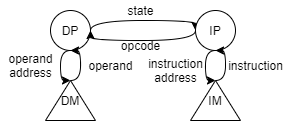
\includegraphics[width=250px]{images/2_Tassonomia_di_Flynn/SISD.png}
\end{figure}

\begin{itemize}
    \item DM: è la gerarchia delle memorie che riguardano i dati
    \item IM: è la gerarchia delle memorie che riguardano le istruzioni
    \item DP: è il data processor
    \item IP: è l'instruction processor
\end{itemize}
In questa architettura si esegue una singola istruzione su un singolo dato ad ogni step temporale. E' la tradizionale macchina sequenziale, cioè il modello di Von Neumann.

Spesso i due bus DP-DM e IP-IM sono in realtà lo stesso bus fisico ma multiplexato, ad esempio durante la fase di fetch di una istruzione il bus funge da IP-IM, durante la fase di fetch degli operandi invece DP-DM.

Le memorie sono esclusivamente accedibili dalla relativa unità di processazione!

\subsection{SIMD}
\begin{figure}[H]
    \centering
    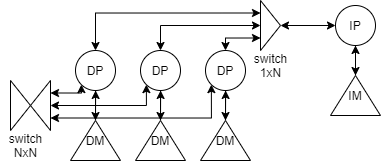
\includegraphics[width=250px]{images/2_Tassonomia_di_Flynn/SIMD.png}
\end{figure}
L' istruzione che IP prende dalla sua memoria è unica e la fornisce a tutti i DP connessi che la eseguiranno sui dati presenti nelle loro memorie.
La connessione che unisce i DP agli IP è comune, passano infatti per uno switch 1 a N, mentre la connessione tra i vari DP può svolgersi in vari modi, così da garantire una specie di connessione punto-punto. Questa connessione può essere utile per scambiarsi i dati delle elaborazioni in quanto ogni DP può accedere direttamente solo ed esclusivamente alla sua DM. La topologia per ottenere questa struttura può seguire vari metodi diversi in base all'utilizzo ed al costo.

Queste strutture sono vere e proprie macchine di calcolo parallelo, permettono:
\begin{itemize}
    \item \emph{parallelismo temporale}: fasi diverse di un'unica istruzione sono eseguite in parallelo in differenti moduli connessi in cascata, praticamente il funzionamento di una pipeline
    \item \emph{parallelismo spaziale}: stessi passi su un array di diversi processori, tutti coordinati da un solo controllore
\end{itemize}

Alcuni esempi sono i super computer vettoriali che svolgono gli stessi calcoli su un ampio dataset, una applicazione importante è quella del calcolo matriciale: la somma o il prodotto di grandi matrici può essere suddiviso in sotto-task e distribuito sulla potenza di calcolo disponibile, infine si uniscono i risultati parziali per ottenere il risultato definitivo.

In questo genere di macchine le periferiche sono connesse alla DM della singola macchina a costituire una sorgente di dati.

\subsection{MISD}
Sono macchine che applicano diverse istruzioni sullo stesso flusso di dati.

Non ci sono importanti applicazioni pratiche per queste macchine se non una diversa interpretazione del meccanismo della pipeline in quanto se interpretiamo l'istruzione fetchata come il dato da elaborare abbiamo diversi circuiti che eseguono diverse istruzioni: fetch, decode, execute.

\subsection{MIMD}
Abbiamo più unità di elaborazione che eseguono ognuna un' operazione diversa. In base a come strutturiamo la memoria dei dati possiamo dividerle in due sotto-categorie.

\subsubsection{DM-MIMD}
Sono macchine MIMD con memoria distribuita:
\begin{figure}[H]
    \centering
    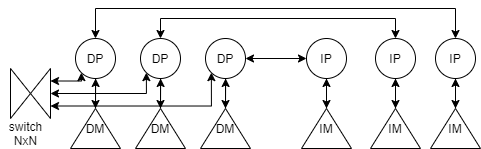
\includegraphics[width=250px]{images/2_Tassonomia_di_Flynn/DM-MIMD.png}
\end{figure}
ogni coppia IP-DP e relative memorie la possiamo vedere come una singola macchina SISD, che comunica con le altre attraverso questa rete fornita dallo switch NxN.

Un esempio pratico è quello delle reti di multicomputers che comunicano attraverso protocolli di scambio di messaggi.

Sono macchine con elevata scalabilità in quanto basta aggiungere una nuova unità SISD, spesso con costo ridotto, per aumentare la capacità di calcolo.

Questa struttura va bene se la rete è veloce, altrimenti il tempo guadagnato distribuendo può essere perso in comunicazione.

Una struttura a cluster di workstation è una tipica applicazione di questa architettura.
Questa struttura comporta una alta disponibilità in quanto se un singolo nodo va giù il suo lavoro può essere distribuito sugli altri presenti con poco o nessun downtime.
Si può anche implementare una logica di \emph{load-balancing} con la quale distribuire il carico sui nodi meno occupati.

\subsubsection{SM-MIMD}
Sono macchine MIMD con la memoria condivisa:
\begin{figure}[H]
    \centering
    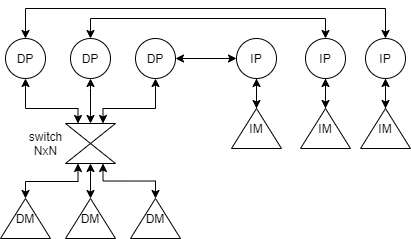
\includegraphics[width=250px]{images/2_Tassonomia_di_Flynn/SM-MIMD.png}
\end{figure}
la comunicazione tra le unità avviene attraverso la memoria condivisa stessa.
Questa struttura si può ottenere all'interno di una macchina con più processori ed una sola memoria principale.
Lo switch deve essere \emph{molto} performante per gestire tutte le richieste delle varie unità di calcolo.

Ha una scalabilità molto ridotta dovuta più che altro alla velocità dello switch e della memoria stessa.

\subsection{Considerazioni}
\begin{itemize}
    \item le macchine SIMD richiedono meno hardware perché concentrano il controllo su una singola unità, tuttavia l'hardware richiesto spesso è custom e quindi più costoso rispetto ai MIMD che permettono l'utilizzo di processori general-purpose
    
    \item le macchine SIMD usano meno memoria delle MIMD perché il programma è presente in singola copia
    
    \item le macchine MIMD sono più flessibili data la loro struttura modulare
\end{itemize}

\subsection{Topologie di connessione}
Abbiamo detto che la comunicazione tra le varie unità è importante, mostriamo alcune delle topologie usate. Definiamo come \emph{grado} il numero di connessioni dirette su un nodo. Definiamo come \emph{diametro} la massima distanza tra due nodi.

\subsubsection{Bus}
\begin{figure}[H]
    \centering
    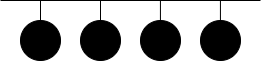
\includegraphics[width=250px]{images/2_Tassonomia_di_Flynn/Bus-topology.png}
\end{figure}

\begin{itemize}
    \item grado dei nodi: 1
    \item diametro della rete: 1
    \item numero di link: 1
    \item tolleranza ai guasti: se un nodo cade la rete non viene intaccata
    \item note: la configurazione è semplice ed affidabile, tuttavia c'è una grande competizione per l'accesso al media, quindi non è molto scalabile
\end{itemize}

\subsubsection{Linear array}
\begin{figure}[H]
    \centering
    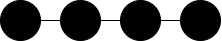
\includegraphics[width=250px]{images/2_Tassonomia_di_Flynn/linear_array-topology.png}
\end{figure}

\begin{itemize}
    \item grado dei nodi: 1 per gli estremi, 2 per tutti gli altri
    \item diametro della rete: N-1
    \item numero di link: N-1
    \item tolleranza ai guasti: se un nodo cade la rete viene partizionata
    \item note: la competizione per l'accesso al mezzo è al minimo possibile, possono esserci fino a $\frac{N}{2}$ comunicazioni in contemporanea ma i nodi devono avere capacità di routing
\end{itemize}

\subsubsection{Ring}
\begin{figure}[H]
    \centering
    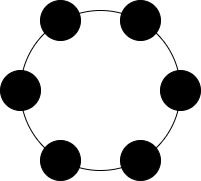
\includegraphics[width=200px]{images/2_Tassonomia_di_Flynn/ring-topology.png}
\end{figure}

\begin{itemize}
    \item grado dei nodi: 2
    \item diametro della rete: $\frac{N}{2}$
    \item numero di link: N
    \item tolleranza ai guasti: se cade un solo nodo la rete non viene intaccata
\end{itemize}

\subsubsection{Full mesh}
\begin{figure}[H]
    \centering
    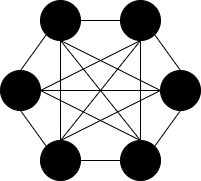
\includegraphics[width=200px]{images/2_Tassonomia_di_Flynn/full_mesh-topology.png}
\end{figure}

\begin{itemize}
    \item grado dei nodi: N-1
    \item diametro della rete: 1
    \item numero di link: $\frac{N \cdot (N - 1)}{2}$
    \item tolleranza ai guasti: massima, se uno qualsiasi dei nodi cade non succede niente alla rete
    \item note: è difficilmente scalabile
\end{itemize}

\subsubsection{B-Tree}
\begin{figure}[H]
    \centering
    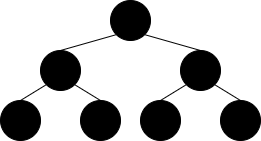
\includegraphics[width=200px]{images/2_Tassonomia_di_Flynn/B_Tree-topology.png}
\end{figure}

\begin{itemize}
    \item grado dei nodi: per la radice 2, per le foglie 1, il resto 3
    \item diametro della rete: $2 \cdot (altezza - 1)$
    \item numero di link: N-1
    \item tolleranza ai guasti: dipende quale punto della rete cade, comunque \\ l' albero viene sempre partizionato se non è una foglia
    \item note: i rami alti sono a rischio di congestione perché di lì passa molto più traffico degli altri link. E' poco scalabile perché dopo un po' il diametro aumenta molto
\end{itemize}

\subsubsection{Star}
\begin{figure}[H]
    \centering
    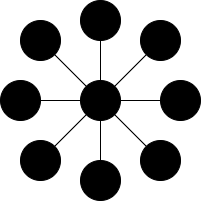
\includegraphics[width=150px]{images/2_Tassonomia_di_Flynn/star-topology.png}
\end{figure}

\begin{itemize}
    \item grado dei nodi: centrale N-1, il resto 1
    \item diametro della rete: 1
    \item numero di link: N-1
    \item tolleranza ai guasti: il centro è un \emph{single point of failure}, ma se cade uno qualsiasi degli altri nodi non c'è nessun problema
\end{itemize}

\subsubsection{Mesh}
\begin{figure}[H]
    \centering
    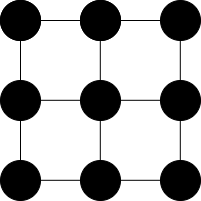
\includegraphics[width=150px]{images/2_Tassonomia_di_Flynn/mesh-topology.png}
\end{figure}

\begin{itemize}
    \item grado dei nodi: 2 per i vertici, 3 per i centrali ai lati, 4 per il resto
    \item diametro della rete: $2 \cdot (raggio -1)$
    \item numero di link: $2 \cdot N - 2 \cdot raggio$
    \item tolleranza ai guasti: buona, devono cadere molti nodi per partizionare la rete
\end{itemize}
NB: il raggio è il lato.

\subsubsection{Toro}
\begin{figure}[H]
    \centering
    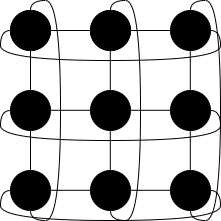
\includegraphics[width=150px]{images/2_Tassonomia_di_Flynn/torus-topology.png}
\end{figure}

\begin{itemize}
    \item grado dei nodi: 4
    \item diametro della rete: $2 \cdot \frac{raggio}{2}$
    \item numero di link: $2 \cdot N$
    \item tolleranza ai guasti: ottima
    \item note: facilmente scalabile
\end{itemize}

\subsubsection{Ipercubo}
\begin{figure}[H]
    \centering
    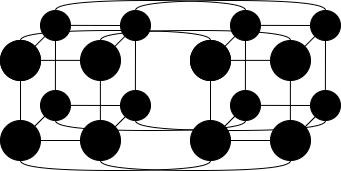
\includegraphics[width=200px]{images/2_Tassonomia_di_Flynn/ipercubo-topology.png}
\end{figure}

\begin{itemize}
    \item grado dei nodi: uguale al raggio
    \item diametro della rete: uguale al raggio
    \item numero di link: $raggio \cdot \frac{N}{2}$
    \item tolleranza ai guasti: ottima
    \item note: scalabile solo con nodi in numero di una potenza di 2
\end{itemize}

\subsection{Metriche di prestazione}
\subsubsection{Speed-up}
E' un coefficiente che indica il guadagno di velocità che si ottiene rispetto ad una esecuzione su uniprocessore.
L'ideale sarebbe avere una relazione lineare nel numero dei processori ($N$) tuttavia si ha sempre $S < N$.
$$ S = \frac{T_1}{T_N} $$

\subsubsection{Efficienza}
$$ E = \frac{S}{N} $$

\subsubsection{Realtà}
Nella realtà abbiamo che non è mai possibile arrivare ad una efficienza unitaria perché ogni algoritmo ha intrinsecamente una componente sequenziale che non si può parallelizzare, questo fenomeno è noto come \emph{Legge di Amdahl}.
Possiamo ridefinire lo speed-up:
$$ S = \frac{T_1}{T_{seq} + \frac{T_1 - T_{seq}}{N}} $$
Man mano che $N$ diventa grande questa quantità tende a $\frac{T_1}{T_{seq}}$, quindi mai lineare con $N$!

In fine bisogna riuscire a tenere alto lo sfruttamento delle CPU per ottenere il massimo rendimento.

